\documentclass[a4paper,12pt]{article} %style de document
\usepackage[utf8]{inputenc} %encodage des caractères
\usepackage[french]{babel} %paquet de langue français
\usepackage[T1]{fontenc} %encodage de la police
\usepackage[top=2cm,bottom=2cm,left=2cm,right=2cm]{geometry} %marges
\usepackage{graphicx} %affichage des images
\usepackage{amssymb}
\usepackage{url}
\usepackage{verbatim}
\usepackage{amsmath}
\usepackage{hyperref}

\begin{document} %début du document

%----------------------------------
%page de garde
%----------------------------------

\begin{titlepage}

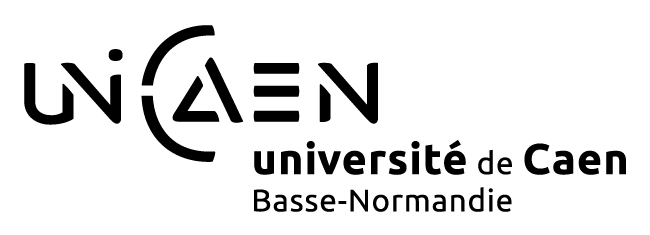
\includegraphics[scale=0.3]{images/unicaen.png}

\vspace{7cm}

\begin{center}

\begin{Huge}
TPA\\
Rapport de Projet\\
\end{Huge}
\vspace{2cm}
\begin{large}
Beauchamp Aymeric 21301016\\
Chagneux Dimitri 21606807\\
Mori Baptiste 21602052\\
Leblond Valentin 21609038\\
\vspace{1cm}
L2-Info-groupe-4A
\end{large}

\end{center}
\end{titlepage}


%------------------------------
%sommaire
%------------------------------

\newpage

\tableofcontents

\newpage

%------------------------------
%contenu
%------------------------------


\section*{Objectifs}
\addcontentsline{toc}{section}{Objectifs}

\subsection*{Description du Sokoban}
\addcontentsline{toc}{subsection}{Description du Sokoban}

Le Sokoban est un jeu de réflexion de type puzzle où le joueur doit placer des caisses sur des objectifs placés à l'avance sur la carte. Le joueur gagne si toutes les caisses sont placées sur les objectifs et il ne peut pousser qu'une seule caisse à la fois. Il existe de nombreux niveaux dont la difficulté est variante.

\begin{figure}[!h]
\centering
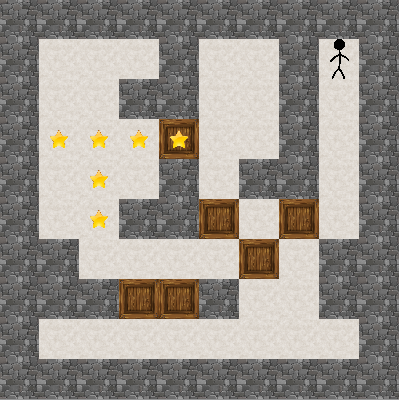
\includegraphics[scale=0.5]{images/sokoban.png}
\caption{Niveau du Sokoban}
\end{figure}

\subsection*{Les fonctionnalités attendues}
\addcontentsline{toc}{subsection}{Les fonctionnalités attendues}

Pour ce projet, nous devions mettre au point une version jouable pour un humain en console, en prenant en compte l'importation de niveaux (au format \textbf{.xsb}). Il était également demandé de réaliser une interface graphique et une fonctionnalité permettant une résolution automatique de niveau.\\
Enfin, permettre de faire jouer en parallèle un humain et un ordinateur, et rendre \textit{anytime} l'algorithme de l'intelligence artificielle. C'est à dire le fait que lorsque le joueur fait un mouvement, l'intelligence artificielle doit en faire un.


\section{Fonctionnalités implémentées}

\subsection{Description des fonctionnalités}

\subsubsection*{Attendues}
\addcontentsline{toc}{subsubsection}{Attendues}

La version console fonctionne à l'aide de saisies de l'utilisateur qui lui permettent de contrôler le jeu. Une fois un niveau terminé, on demande au joueur si il souhaite passer au niveau suivant.\\

La carte est chargée à partir d'un fichier \textbf{.xsb} contenant des lignes de caractères, que l'on transforment en liste de caractères.\\
La carte est donc modélisée par des chaînes de caractères:
\begin{itemize}
\item \textbf{\#} pour un mur
\item \textbf{\$} pour une caisse
\item \textbf{@} pour le joueur
\item \textbf{.} pour un objectif
\item \textbf{*} pour une caisse sur un objectif
\item \textbf{+} pour le joueur sur un objectif
\item \textbf{espace} pour les cases vides
\end{itemize}

\begin{figure}[!h]
\centering
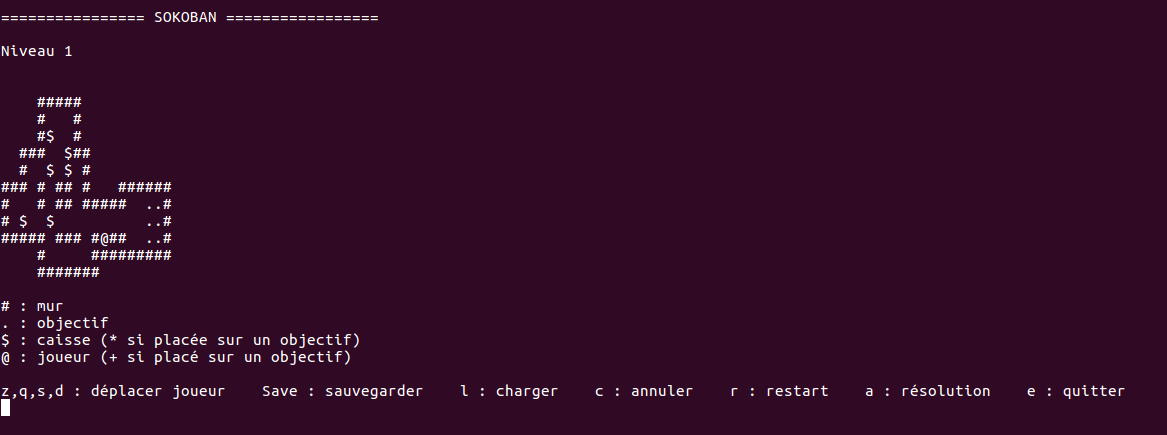
\includegraphics[scale=0.5]{images/Capture.png}
\caption{Interface console}
\end{figure}

Au niveau de l'interface graphique, nous avons une zone de jeu dans laquelle on dessine le niveau et des boutons pour gérer les différentes fonctionnalités. Le personnage est déplaçable avec les flèches directionnelles ou ZQSD, si le joueur a bloqué une caisse ou si il a gagné, il ne peut plus bouger et doit recommencer le niveau ou passer au suivant (seulement si il a gagné). Si le joueur gagne, le personnage effectue le Dab et si il perd, le personnage pleure.


\begin{figure}[!h]
\centering
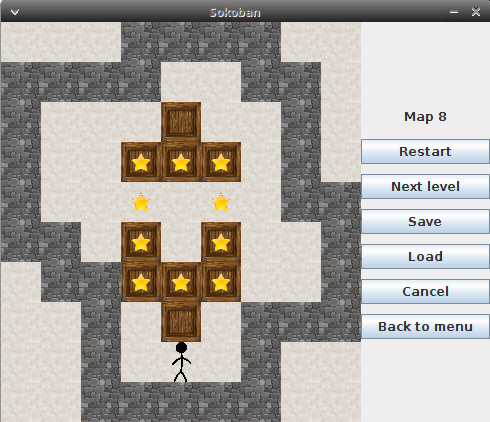
\includegraphics[scale=0.5]{images/Capture2.png}
\caption{Interface graphique}
\end{figure}

\subsubsection*{Ajoutées}
\addcontentsline{toc}{subsubsection}{Ajoutées}

Au lancement du programme, l'utilisateur peut choisir un profil ou en créer un nouveau.\\
En fonction de l'avancement du profil donné, le joueur a débloqué un certain nombre de carte, pour débloquer la carte suivante il faut finir le niveau en cours. Lorsqu'un profil est chargé, la dernière carte non terminée est lancée automatiquement.\\

Nous proposons également à l'utilisateur de sauvegarder sa partie à un instant du niveau donné, de charger sa sauvegarde (il n'y a pas de conflit entre la sauvegarde de chaque utilisateur), d'annuler le coup précédemment joué (cette fonctionnalité n'annule qu'un seul coup en arrière) et enfin de recommencer le niveau courant.

\subsection{Organisation du projet}

Pour le début du projet, nous avons tous travaillés ensemble sur la création de la structure de base du jeu sur comment on va représenter chaque éléments qui composent le jeu (joueur, case vide, caisse ou encore la carte qui les contiendra). Ensuite nous nous sommes interrogé sur la manière de déplacer le joueur ainsi que faire pousser les caisse par le joueur et faire en sorte de gérer les collisions avec les murs.\\
Nous avons rencontrés des difficultés pour la détection d'une caisse qui est bloqué, nous avons d'abord dit qu'une caisse est bloquée si elle se trouve entre deux murs qui se trouve sur deux axes différents (cas de gauche de la \textbf{figure \ref{figure4}}). Nous nous sommes rendu vite compte que ce n'était pas le seul cas de caisse bloquée, comme on peut le voir sur la deuxième image de la \textbf{figure \ref{figure4}}, on ne peut déplacer aucune des deux caisses car elles se bloquent entre elles, nous avons donc gérer ce cas mais même en fin de projet nous avions oubliés certains cas de caisses bloquées (le fait d'avoir un amas de caisse rendait la détection plus compliquée et les cas étaient particuliers).

\begin{figure}[!h]
\centering
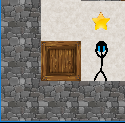
\includegraphics[scale=0.5]{images/Capture3.PNG}
\hspace{1cm}
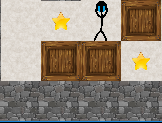
\includegraphics[scale=0.5]{images/Capture4.png}
\caption{Blocage simple de caisse(s)}
\label{figure4}
\end{figure}

Ensuite, nous nous sommes séparés en trois groupes, deux d'entre nous se sont lancés sur l'IA avec l'algorithme A*, puis une autre personne s'est lancée dans la création d'un main et toute la gestions de fichiers (sauvegarde, chargement, traduction entre une carte enregistré dans un fichier et notre représentation d'un niveau de notre code). Enfin la dernière personne s'est occupée de gérer des cas plus complexes de détections de caisses bloquées puis est partie dans la mis en place de l'interface graphique.

L'interface graphique ayant bien avancé, des nouvelles fonctionnalités ont étaient ajoutées dans celle-ci et des réglages dans la manière de sauvegarder une map a était changé ce qui a posé un problème au niveau du main qui faisait fonctionner le jeu en version console, celle-ci n'était plus à jour il a fallut donc revoir notre main de la console pour qu'elle la fonctionnalité de sélection de profils qui a était implémenté d'abord en version graphique, changer la manière de sauvegarder une map car dans la première version, la méthode ne nous permettait pas de recommencer le niveau courant.\\

Au niveau de l'IA, nous avions réussi assez tardivement à faire résoudre une grande partie de nos maps en quelques secondes, en effet nous avions rencontré pas mal de problèmes en ce qui concerne les choix que doit effectuer l'IA et de comprendre pourquoi elle ne faisait pas ce que l'on attendait.

\section{Éléments techniques}

\section{Architecture du projet}

\section{Expérimentations et usages}

\section*{Conclusion}
\addcontentsline{toc}{section}{Conclusion}


\end{document}

